\usetikzlibrary{shapes,arrows}
\usetikzlibrary{positioning}
\usetikzlibrary{calc,shapes.callouts,shapes.arrows}

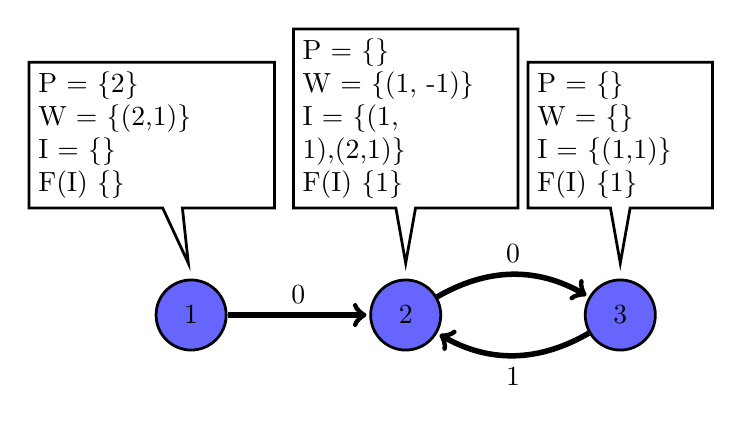
\begin{tikzpicture}[node distance = 1.8cm, auto]


\tikzstyle{operator} = [circle, draw, fill=blue!60, text width=1.5em, text centered, line width=1pt]

    \node [operator] at (0, 0) (1) {1};
    \node[draw, rectangle callout, above = of 1, line width=1pt, text width=8.2em, callout relative pointer={(0.2cm,-0.7cm)},above= 25pt, shift={(-0.5,0)}] 
   { 
     P = \{2\}\\
     W = \{(2,1)\}\\
     I = \{\}\\
     F(I) \{\}
    };

    \node [operator, right = of 1] (2) {2};
     \node[draw, rectangle callout, above = of 2, line width=1pt, text width=7.45em, callout relative pointer={(0cm,-0.7cm)},above= 25pt] 
   { 
     P = \{\}\\
     W = \{(1, -1)\}\\
     I = \{(1, 1),(2,1)\}\\
     F(I) \{1\}
    };

    \node [operator, right = of 2] (3) {3}; 
     \node[draw, rectangle callout, above = of 3, line width=1pt, text width=6em, callout relative pointer={(0cm,-0.7cm)},above= 25pt] 
   { 
     P = \{\}\\
     W = \{\}\\
     I = \{(1,1)\}\\
     F(I) \{1\}
    };


    \draw [thick,->,shorten >=1pt, line width=2pt] (1) edge node {0} (2); 
    \draw [thick,->,shorten >=1pt, line width=2pt] (2) edge  [bend left]  node {0} (3);
     \draw [thick,->,shorten >=1pt, line width=2pt] (3) edge  [bend left]  node {1} (2); 


\end{tikzpicture}
